% --------------------------------------------------------------
% This is all preamble stuff that you don't have to worry about.
% Head down to where it says "Start here"
% --------------------------------------------------------------
 
\documentclass[12pt]{article}
 
\usepackage[margin=1in]{geometry} 
\usepackage{bm} % bold in mathmode \bm
\usepackage{amsmath,amsthm,amssymb,mathtools}
\usepackage{dsfont} % for indicator function \mathds 1
\usepackage{mathdots} % for \iddots
\usepackage{tikz,pgf,pgfplots}
\usepackage{enumerate} 
\usepackage[multiple]{footmisc} % for an adjascent footnote
\usepackage{graphicx,float} % figures
\usepackage{framed} % surround a text with a box 
\usepackage{changepage} % \begin{adjustwidth}{2cm}{} environment

\newtheorem{definition}{Definition}
\let\olddefinition\definition
\renewcommand{\definition}{\olddefinition\normalfont}
\newtheorem{lemma}{Lemma}
\let\oldlemma\lemma
\renewcommand{\lemma}{\oldlemma\normalfont}
\newtheorem{proposition}{Proposition}
\let\oldproposition\proposition
\renewcommand{\proposition}{\oldproposition\normalfont}
\newtheorem{corollary}{Corollary}
\let\oldcorollary\corollary
\renewcommand{\corollary}{\oldcorollary\normalfont}
\newtheorem{theorem}{Theorem}
\let\oldtheorem\theorem
\renewcommand{\theorem}{\oldtheorem\normalfont}

%%% PLOTTING PARAMETERS
\tikzstyle{bag} = [text width=7em, text centered] %% binomial tree node width
\tikzstyle{end} = []

\pgfplotsset{soldot/.style={color=black,only marks,mark=*},
             holdot/.style={color=black,fill=white,only marks,mark=*},
             compat=1.12}
%%%

%% I want to be in control of when to indent...
%% set noindent as the default status and define \indent to indent a line
\newlength\tindent
\setlength{\tindent}{\parindent}
\setlength{\parindent}{0pt}
\renewcommand{\indent}{\hspace*{\tindent}}

\newcommand*{\vv}[1]{\vec{\mkern0mu#1}} % \vec command

%% DAVIDS MACRO KIT %%
\newcommand{\R}{\mathbb R}
\newcommand{\N}{\mathbb N}
\newcommand{\Z}{\mathbb Z}
\renewcommand{\P}{\mathbb P}
\newcommand{\Q}{\mathbb Q}
\newcommand{\E}{\mathbb E}
\newcommand{\var}{\mathrm{Var}}
\newcommand{\Var}{\mathrm{Var}}
\newcommand{\cov}{\mathrm{Cov}}
\newcommand{\Cov}{\mathrm{Cov}}
\newcommand{\indist}{\,{\buildrel \mathcal D \over \sim}\,}

\newcommand{\bigtau}{\text{{\large $\bm \tau$}}}

\begin{document}
 
% --------------------------------------------------------------
%                         Start here
% --------------------------------------------------------------
 
\title{Mathematical \& Computational Finance I\\Lecture Notes}
\author{Random Walks \& Perpetual Options}
\date{March 17 2016 \\ Last update: \today{}}
\maketitle

% SECTION: 
\section{Reflection Principle}

\begin{theorem} {\bf Reflection Principle.}\footnote{I still don't quite see this... Maybe it's less interesting than I am imagining.} If $a, b > 0$ then
\begin{equation*}
	N^0_n(a, b) = N_n(-a,b)
\end{equation*}

\indent That is, the number of paths from $(0,a)$ to $(n,b)$ that touch/cross the $x$-axis is identical to the number of paths from $(0,-a)$ to $(n,b)$.

\begin{proof} Each path from $(0, -a)$ to $(n,b)$ must intersect the $x$ axis at some first point $(k,0)$. We reflect the segment of the path between time 0 and time $k$ about the $x$-axis in order to obtain the original walk from $(0,a)$ to $(n, b)$. \\

\indent This operation gives us a one-to-one correspondence between both collections of paths. So, the number of paths from $(0, a)$ that reach $b$ at time $n$ is identical to those\footnote{I think I'm forgetting something relating to the difference between $N^0_n(a,b)$ and $N_n(a,b)$.} starting from $(0, -a)$, as desired.

\begin{figure}[H]
\centering
\begin{tikzpicture}
\begin{axis}[thick,
	height=10cm, width=14cm,
    axis lines=middle,
    xmin=0, xmax=15,
    ymin=-6, ymax=6,
    xlabel={$x$}, ylabel={$M$},
    ticks = none,
    xlabel style={at=(current axis.right of origin), anchor=west}, 
    ylabel style={at=(current axis.above origin), anchor=south}
]
	\addplot [only marks] coordinates {(0,5)(1,4)(2,5)(3,4)(4,3)(5,2)(6,1)(7,0)(8,-1)(9,0)(10,1)(11,0)(12,1)(13,2)};
	\addplot [only marks] coordinates {(0,-5)(1,-4)(2,-5)(3,-4)(4,-3)(5,-2)(6,-1)};
	\draw (0,5) node	 [above right] {$(0,a)$};
	\draw (0,5) -- (1,4);
	\draw (1,4) -- (2,5);
	\draw (2,5) -- (8,-1);
	\draw (8,-1) -- (10,1);
	\draw (10,1) -- (11,0);
	\draw (11,0) -- (13,2) node[above right] {$(n,b)$};
	%% reflected walk
	\draw (0,-5) node [below right] {$(0,-a)$};
	\draw[thin, gray!80] (0,-5) -- (1,-4);
	\draw[thin, gray!80] (1,-4) -- (2,-5);
	\draw[thin, gray!80] (2,-5) -- (7,0);
	%%
	\draw[ultra thin] (7,0) -- (7,2) node [above] {$k$};
\end{axis}
\end{tikzpicture}
\caption{Example of the Reflection Principle with the random walk reflected at the first point of contact with the $x$-axis, point $(k,0)$.}
\end{figure}
\end{proof}
\end{theorem}

\begin{corollary} {\bf Ballot Theorem.}\footnote{To do: I'm not sure I follow the argumentation...} If $b > 0$ then the number of possible paths from $(0,0$ to $(n,b)$ which do not revisit the $x$-axis is
\begin{equation*}
	\frac{b}{n} N_n(0,b)
\end{equation*}

\begin{proof} The first step of all paths must be\footnote{This is the case because we finish $b > 0$ in the positive quadrant.} $(1,1)$ and so the number of possible paths is\footnote{$N_{n - 1}(1,b)$ denotes the number of paths of length $n - 1$ from $(1, 1)$ to $(b, n)$, and $N^0_{n - 1}(1, n)$ denotes the number of paths from $(1,1)$ to $(n,n)$ that touch/cross the $x$-axis.}~\footnote{Should the terms in the first line of the equality be $N^0_{n - 1}(1,b)$ and $N_{n - 1}(-1,b)$ instead of the present $N^0_{n - 1}(1,n)$ and $N_{n - 1}(-1,n)$?}
\begin{align*}
	N_{n - 1}(1,b) - N^0_{n - 1}(1,n) &= N_{n - 1}(1, b) - N_{n - 1}(-1, n) \quad \text{(reflection principle)} \\
	&= \frac{b}{n}N_n(0,b)
\end{align*}

where the final equality follows since\footnote{To do: Actually compute these to convince myself that this is so.}
\begin{equation*}
	\frac{n - 2r}{n}{{n}\choose{r}} = {{n - 1}\choose{r}} - {{n - 1}\choose{r - 1}}
\end{equation*}

for $r = 1,2,...,n-1$ and if we use the fact we had found before that
\begin{equation*}
	N_n(a,b) = {{n}\choose{\frac{1}{2}(n - b + a)}}
\end{equation*}

then $r = \frac{1}{2}(n - b)$.
\end{proof}
\end{corollary}

\underline{Example:} {\em (Ballot Theorem).} Suppose Donald and Hillary are in an election and that Donald wins by $b$ votes in $n$ ballots cast, where ballots are counted in a random order. Then
\begin{align*}
	\P(\text{Donald leads throughout the count)} &= \frac{ \#\{\text{Paths in which Donald leads throughout}\} } { \#\{\text{All paths}\} } \\
	&= \frac{ \frac{b}{n} N_n(0,b) }{  N_n(0,b)} \\
	&= \frac{b}{n}
\end{align*}

\underline{Example:} {\em  (Exercise 5.4 -- Distribution of $\tau_2$).} Consider a symmetric random walk. Let $\tau_2$ denote the first time the random walk, starting from $m = 0$, reaches level 2. Now, recall that we had the probability generating function
\begin{equation*}
	\E[\alpha^{\tau_2}] = \left( \frac{1 - \sqrt{1 - \alpha^2}}{ \alpha } \right)^2
\end{equation*}

for all $\alpha \in (0,1)$. Using the power series expansion we were able to write
\begin{align*}
	\left( \frac{1 - \sqrt{1 - \alpha^2}}{ \alpha } \right)^2 &= \frac{ (1 - \sqrt{1 - \alpha^2})^2 }{ \alpha^2 } \\
	&= \frac{ 1 - 2\sqrt{1 - \alpha^2} + 1 - \alpha^2 }{ \alpha^2 } \\
	&= \frac{ 2 - 2\sqrt{1 - \alpha^2} }{ \alpha^2 } - 1 \\
	&= \frac{2}{\alpha} \cdot \frac{1 - \sqrt{1 - \alpha^2}}{\alpha} - 1 \\
	&= -1 + \frac{2}{\alpha} \sum^\infty_{j = 1} \left( \frac{1}{2} \right)^{2j - 1} \frac{(2j - 2)!}{j!(j - 1)!} \left(\alpha^2\right)^j \\
	&= -1 + \sum^\infty_{j = 1} \left( \frac{\alpha}{2} \right)^{2j - 2} \frac{(2j - 2)!}{j!(j - 1)!} \\
	&= \sum^\infty_{j = 2} \left( \frac{\alpha}{2} \right)^{2j - 2} \frac{(2j - 2)!}{j!(j - 1)!} \\
	&= \sum^\infty_{k = 1} \left(\frac{\alpha}{2}\right)^{2k} \frac{(2k)!}{(k + 1)!k!} 
\end{align*}

{\bf (i)} Use the power series above to determine $\P\{(\tau_2 = 2k)\}$, $k = 1,2,...$ \\

\underline{Solution:} Note that the random walk can only reach level two on an even number of steps so that we have $\P(\tau_2 = 2k - 1) = 0$ for $k = 1,2,...$. Then
\begin{equation*}
	\E[\alpha^{\tau_2}] = \sum^\infty_{k = 1} \alpha^{2k} \P(\tau_2 = 2k)
\end{equation*}

Equating this terms of the series from result with the terms of the series expansion above
\begin{align*}
	\alpha^{2k} \P(\tau_2 = 2k) &= \left(\frac{\alpha}{2}\right)^{2k} \frac{(2k)!}{(k + 1)!k!} \\
\implies \P(\tau_2 = 2k) &= \left(\frac{1}{2}\right)^{2k} \frac{(2k)!}{(k + 1)!k!}
\end{align*}

{\bf (ii)} Use the reflection principle to determine $\P(\{\tau_2 = 2k\})$ for $k = 1,2,...$ \\

\underline{Solution:} Denote $N_n(a,b)$ to be the number of paths from $(0,a)$ to $(n,b)$. The sum of the number of up steps, $r$, and down steps, $l$, must be the total number of steps $n$
\begin{equation*}
	r + l = n
\end{equation*}

\indent We also require the difference between the up and down steps (net upward movement) be $b - a$ 
\begin{equation*}
	r - l = b - a
\end{equation*}

Solving this system for $r$ and $l$
\begin{align*}
	r &= \frac{1}{2}(n + (b - a)) \\
	l &= \frac{1}{2}(n - (b - a))
\end{align*}

So then the number of paths $N_n(a,b)$
\begin{equation*}
	N_n(a,b) = {{n}\choose{r}} 
\end{equation*}

can be rewritten as
\begin{equation*}
	N_n(a,b) = {{n}\choose{\frac{n + b - a}{2}}}
\end{equation*}

and
\begin{align*}
	\P(M_n = b ~|~ M_0 = 0) &= N_n(a,b) p^r q^l \\
	&= {{n}\choose{\frac{n + b - a}{2}}} p^r q^l \\
	&= {{n}\choose{\frac{n + b - a}{2}}} p^{ \frac{1}{2}(n + (b - a)) } q^{ \frac{1}{2}(n - (b - a)) }
\end{align*}

\indent For $a,b > 0$ let $N^0_n(a,b)$ be the number of paths from $(0,a)$ to $(n,b)$ that touch/cross the $x$-axis. Each path from the point $(0,-a)$ to $(n,b)$ must intersect the $x$-axis at some earliest point $(k,0)$. \\

\indent If we reflect this segment of the walk along $0$ to $k$ about the $x$-axis we obtain a walk joining $(0,a)$ to $(n,b)$ which intersects (touch/cross) the $x$-axis at $(k,0)$. This operation gives us a one-to-one correspondence between both collection of walks. This gives us the \underline{Reflection Principle}
\begin{equation*}
	N^0_n(a,b) = N_n(-a,b) \quad a,b > 0
\end{equation*}

\indent If $b > 0$ then the number of paths from node $(0,0)$ to $(n,b)$ which to not revisit the $x$-axis (revisit after its initial contact at $(0,0)$) is, since the first step must be to $(1,1)$ by construction,
\begin{align*}
	N_{n - 1}(1,b) - N^0_{n - 1}(1,b) &= N_{n - 1}(1,b) - N_{n - 1}(-1,b) \\
	&= {{n - 1}\choose{r}} - {{n - 1}\choose{r - 1}} \\
	&= \frac{ n - 2r }{ n } {{n}\choose{r}} \\
	&= \frac{b}{n} N_n(0,b) \quad \text{\bf (Ballot Theorem)}
\end{align*}

Suppose the first $n$ steps of the random walk are given by 
\begin{equation*}
	\left\{0, X_1, X_1 + X_2, \cdots, \sum^n_{j = 1} X_j \right\}
\end{equation*}

and that the random walk hits the value $b$ for the first time on the $n^\text{th}$ step. We say that the \underline{reversed random walk} given by
\begin{equation*}
	\left\{0, X_n, X_n + X_{n - 1}, \cdots, \sum^n_{j = 1} X_j \right\}
\end{equation*}

starts at $0$, will never return the $x$-axis, and hits $b$ on the final step. Hence, the probability of the first hitting time of level $b$ occurring on step $n$ is\footnote{From what is this motivated by?}
\begin{equation*}
	\frac{b}{n}N_n(0,b) p^{\frac{1}{2}(n + b)} q^{\frac{1}{2}(n - b)}
\end{equation*}

Applying the above result for $n = 2k, p = \frac{1}{2}$ and $b = 2$ we find
\begin{align*}
	\P(\tau_2 = 2k) &= \P(M_{2k} = 2, M_{2k - 1} \neq 2,..., M_1 \neq 2~|~M_0 = 0) \\
	&= \P(M_{2k} = 2, M_{2k - 1} \neq 0,..., M_1 \neq 0~|~M_0 = 0) \\
	&= \frac{2}{2k} {{2k}\choose{\frac{1}{2}(2k - 2)}} p^{\frac{1}{2}(2k + 2)} q^{\frac{1}{2}(2k - 2)} \\
	&= \frac{1}{k} \frac{ (2k)! }{ (k + 1)!(k - 1)! } \left( \frac{1}{2} \right)^{2k} \quad \left(\text{since  } p = q = \frac{1}{2}\right) \\
	&= \frac{ (2k)! }{ (k + 1)!k! } \left( \frac{1}{2} \right)^{2k}
\end{align*}

which agrees with our result from part {\bf (i)}.

\begin{figure}[H]
\centering
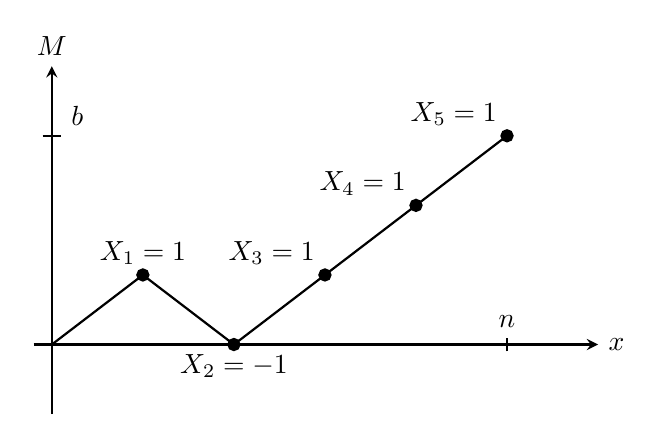
\begin{tikzpicture}
\begin{axis}[thick,
	height=6cm, width=8.75cm,
    axis lines=middle,
    xmin=-0.2, xmax=6,
    ymin=-1, ymax=4,
    xlabel={$x$}, ylabel={$M$},
    ticks = none,
    xlabel style={at=(current axis.right of origin), anchor=west}, 
    ylabel style={at=(current axis.above origin), anchor=south}
]
	\addplot [only marks] coordinates {(1,1)(2,0)(3,1)(4,2)(5,3)};
	\draw (0,0) -- (1,1) node[above] {$X_1 = 1$};	
	\draw (1,1) -- (2,0) node[below] {$X_2 = -1$};
	\draw (2,0) -- (3,1) node[above left] {$X_3 = 1$};	
	\draw (3,1) -- (4,2) node[above left] {$X_4 = 1$};	
	\draw (4,2) -- (5,3) node[above left] {$X_5 = 1$};	
	\draw (5,-0.1) -- (5,0.1) node[above] {$n$};
	\draw (-0.1,3) -- (0.1,3) node[above right] {$b$};
\end{axis}
\end{tikzpicture}
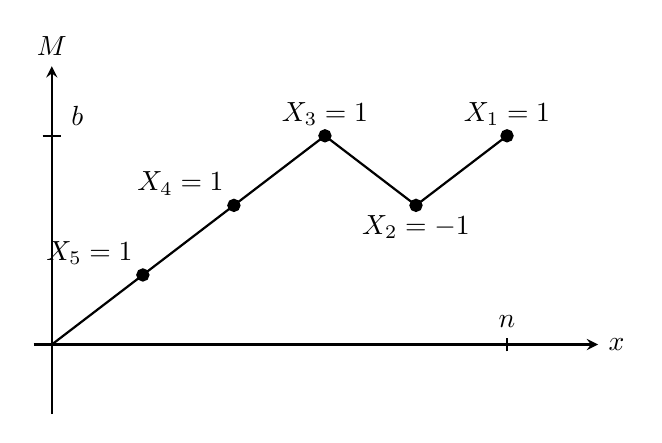
\begin{tikzpicture}
\begin{axis}[thick,
	height=6cm, width=8.75cm,
    axis lines=middle,
    xmin=-0.2, xmax=6,
    ymin=-1, ymax=4,
    xlabel={$x$}, ylabel={$M$},
    ticks = none,
    xlabel style={at=(current axis.right of origin), anchor=west}, 
    ylabel style={at=(current axis.above origin), anchor=south}
]
	\addplot [only marks] coordinates {(1,1)(2,2)(3,3)(4,2)(5,3)};
	\draw (0,0) -- (1,1) node[above left] {$X_5 = 1$};	
	\draw (1,1) -- (2,2) node[above left] {$X_4 = 1$};
	\draw (2,2) -- (3,3) node[above] {$X_3 = 1$};	
	\draw (3,3) -- (4,2) node[below] {$X_2 = -1$};	
	\draw (4,2) -- (5,3) node[above] {$X_1 = 1$};
	\draw (5,-0.1) -- (5,0.1) node[above] {$n$};
	\draw (-0.1,3) -- (0.1,3) node[above right] {$b$};
\end{axis}
\end{tikzpicture}
\caption{Example of a a random walk (left) and its reversed random walk (right). Notice that the reverse walk never crosses/touches the $x$ axis but is still able to reach level $b$ at time $n$.}
\end{figure}

\section{Perpetual American Put Option}

\indent We should first note that these types of derivatives are not actually traded in the real world (at least not in this form). There are other risks (credit, counterparty, etc...) associated with perpetuities that make their trading impractical. These derivatives are a mathematical exercise that produce results which can be applied/extended to more salient instruments. \\

\indent Consider the binomial asset pricing model with $S_0 = 4, r = \frac{1}{4}, u = 2, d = \frac{1}{2}$ and consider an American put option with no expiry date. We have that $\tilde{\P}(\omega_j = H) = \tilde{p} = \frac{1}{2}$. From this we may construct the {\em infinite} binomial tree

\begin{figure}[H]
\centering
\begin{tikzpicture}[sloped]
  \node (a) at (0,0) [bag] {$S_0 = 4$};
  \node (b) at (4,-1.5) [bag] {$S_1(T) = 2$};
  \node (c) at (4,1.5) [bag] {$S_1(H) = 8$};
  \node (d) at (8,-3) [bag] {$S_2(TT) = 1$};
  \node (e) at (8,0) [bag] {$S_2(HT) = S_2(TH) = 4$};
  \node (f) at (8,3) [bag] {$S_2(HH) = 16$};
  \draw (10,-3.5) node {$\ddots$};  
  \draw (10,-3) node {$\cdots$};
  \draw (10,-2.25) node {$\iddots$};
  \draw (10,-0.5) node {$\ddots$};
  \draw (10,0) node {$\cdots$};
  \draw (10,0.75) node {$\iddots$};
  \draw (10,2.5) node {$\ddots$};
  \draw (10,3) node {$\cdots$};
  \draw (10,3.75) node {$\iddots$};
  \draw [->] (a) to node [below] {} (b);
  \draw [->] (a) to node [above] {} (c);
  \draw [->] (c) to node [below] {} (f);
  \draw [->] (c) to node [above] {} (e);
  \draw [->] (b) to node [below] {} (e);
  \draw [->] (b) to node [above] {} (d);
\end{tikzpicture}
\caption{Infinite asset price tree $S_n$.}
\end{figure}

Note that we may write
\begin{equation*}
	S_n = S_02^{M_n}
\end{equation*}

where $M_n$ is a symmetric random walk under the risk-neutral measure $\tilde{\P}$. Assume that we have strike $K = 4$:
\begin{enumerate}[(i)]
	\item At time $n$ the long party has the right to sell the underlying asset worth $S_n$ for $\$4$.
	\item The payoff of such an action is $v(S_n) = 4 - S_n$.
	\item We wish to find a price for this contract in terms of $S_0$.
	\item Since the contract has no expiration it is reasonable to assume that the price, exercise strategy, and hedging strategy should not depend on time.
\end{enumerate}

Consider the following possible exercise strategies: \\

\begin{adjustwidth}{1cm}{} {\bf Policy 0:} Exercise our perpetual option immediately. This corresponds to the first passage time $\tau_0$, the first time $M_n = 0$. Since we have defined $M_0 = 0$ we have that $\tau_0 = 0$ by definition. The value of the option using this exercise strategy is\footnote{Since at time zero we have $S_0 = 4$, so $V^(\tau_0) = K - S_0 = 4 - 4 = 0$.}
\begin{equation*}
	V^{(\tau_0)} = 0
\end{equation*}
\end{adjustwidth}

\begin{adjustwidth}{1cm}{} {\bf Policy 1:} Exercise the first time $S_n$ falls to level $\$2$. This corresponds to exercising the option according to $\tau_{-1}$: The first time\footnote{Since $S_n = S_0 2^{M_n} = 4\cdot 2^{-1} = 2$, so $K - S_n = 4 - 2 = 2$.} $M_n = -1$. We denote the value of this strategy by
\begin{equation*}
	V^{(\tau_{-1})}
\end{equation*}
\end{adjustwidth}

\begin{adjustwidth}{1cm}{} {\bf Policy 2:} Exercise the first time $S_n$ falls to level $\$1$. This corresponds to the exercise strategy of $\tau_{-2}$: The first time $M_n = -2$. We denote the value of this strategy by
\begin{equation*}
	V^{(\tau_{-2})}
\end{equation*}
\end{adjustwidth}

We may generalize this result for positive integers. Let $m$ be a positive integer. 

\begin{adjustwidth}{1cm}{} {\bf Policy $\bm m$:} Exercise the first time $S_n$ falls to level $S_0 2^{-m} = 4\cdot 2^{-m}$. This corresponds to exercising according to fist passage time $\tau_{-m}$: The first time $M_n = -m$. We denote the value of this strategy by
\begin{equation*}
	V^{(\tau_{-m})}
\end{equation*}

\indent We may find this value by computing the risk-neutral value of the put assuming the long part exercises according to $\tau_{-m}$
\begin{align*}
	V^{(\tau_{-m})} &= \tilde{\E} \left[ \left( \frac{1}{1 + r} \right)^{\tau_{-m}} (K - S_{\tau_{-m}}) \right] \\
	&= 4 \left( 1 - 2^{-m} \right) \tilde{\E} \left[ \left( \frac{4}{5} \right)^{\tau_{-m}} \right]
\end{align*}

Now, recall that for $\alpha \in (0,1)$ we had that
\begin{equation*}
	\E \left[ \alpha^{\tau_m} \right] = \left( \frac{1 - \sqrt{1 - \alpha^2}}{ \alpha} \right)^{|m|}
\end{equation*}

So, with $\alpha = \frac{4}{5}$ we get
\begin{align*}
	\tilde{\E} \left[ \left( \frac{4}{5} \right)^{\tau_m} \right] = \left( \frac{1 - \sqrt{1 - \left( \frac{4}{5}\right)^2}}{ \left( \frac{4}{5} \right) } \right)^{|m|} &= \left( \frac{5}{4} \cdot \left[ 1 - \sqrt{ 1 - \frac{16}{25} }\right]  \right)^{m} \\
	&= \left( \frac{5}{4} \cdot \left[ 1 - \sqrt{ \frac{9}{25} } \right] \right)^m \\
	&= \left( \frac{5}{4}\cdot\left[ 1 - \frac{3}{5}\right] \right)^m \\
	&= \left( \frac{5}{4}\cdot\frac{2}{5} \right)^m \\
	&= \left( \frac{1}{2} \right)^m
\end{align*}

Thus, by symmetry
\begin{align*}
	\tilde{\E} \left[ \left( \frac{4}{5} \right)^{\tau_{-m}} \right] &= \left( \frac{1}{2} \right)^m
\end{align*}

Hence
\begin{align*}
	V^{(\tau_{-m})} &= 4 \left( 1 - 2^{-m} \right) \tilde{\E} \left[ \left( \frac{4}{5} \right)^{\tau_{-m}} \right] \\
	&= 4 \left( 1 - 2^{-m} \right)  \left( \frac{1}{2} \right)^m \\
\end{align*}
\end{adjustwidth}

\indent For this value of $V^{(\tau_{-m})} = 4\cdot(1 - 2^{-m}) \left( \frac{1}{2}\right)^m$ we can show that $V^{(\tau_{-m})}$ is in fact a decreasing function for increasing $m$ (decreasing $-m$). In particular,
\begin{align*}
	V^{(\tau_{-1})} &= 4 \left(1 - \frac{1}{2}\right)\frac{1}{2} = 1 \\
	V^{(\tau_{-2})} &= 4 \left(1 - \frac{1}{4}\right)\frac{1}{4} = \frac{3}{4} \\
	V^{(\tau_{-3})} &= 4 \left(1 - \frac{1}{8}\right)\frac{1}{8} = \frac{7}{16} \\
	&\vdots
\end{align*}

\indent Based on these results we suspect that the optimal exercise policy is to exercise the first time $S_n$ falls to $\$2$ (corresponding to $\tau_{-1}$. It is reasonable to assume\footnote{Why?} this result should be independent of the initial stock price $S_0$: Regardless of the initial price the long party should exercise the first time the price reaches level $\$2$ or below. \\

\indent We wish to confirm this optimal strategy. To do so we first determine the price of the contract for different values of $S_0$, under the proposed optimal strategy (exercise the first time we're at or below $\$2$). \\

\indent Suppose $S_0 = 2^j$ for $j \leq 1$. Then $S_0 \leq 2$ and we would exercise immediately according to our strategy. The value of the contract becomes
\begin{equation*}
	v(2^j) = 4 - 2^j, j \leq 1
\end{equation*}

\indent Suppose $S_0 = 2^j$ for $j \geq 2$. We would exercise this strategy the first time we reach $S_n = 2$. That is, we will exercise the first time
\begin{align*}
	2 &\geq S_n \\
	&\equiv S_0 \cdot 2^{M_n} \\
	&= 2^j \cdot 2^{M_n} \\
	&= 2^{j + M_n} \\
	\implies j + M_n &\leq 1 \\ 
	\implies M_n &\leq 1 - j = -(j - 1)
\end{align*}

That is, we exercise the first time $M_n \leq -(j - 1)$. Then, according to our strategy
\begin{align*}
	v(S_n) = v(2^j) &= \tilde{\E} \left[ \frac{1}{(1 + r)^{\tau_{-(j - 1)}}} \left(K - S_{\tau_{-(j - 1)}} \right) \right] \\
	&= \tilde{\E} \left[ \left( \frac{4}{5} \right)^{\tau_{-(j - 1)}} \left( 4 - 2 \right) \right] \\
	&= 2\cdot \tilde{\E} \left[ \left( \frac{4}{5} \right)^{\tau_{-(j - 1)}} \right] \\
	&= 2 \cdot \left( \frac{1}{2} \right)^{j - 1} \\
	&= 2 \cdot \frac{2}{2^j} \\
	&= \frac{4}{2^j} \quad j = 2,3,4,...
\end{align*}

\indent Putting these results together we find that, for $S_0 = 2^j, j \in \Z$, our proposed optimal value for the perpetual put contract is
\begin{equation*}
	v(2^j) =
	\begin{cases}
		4 - 2^j & \text{if } j \in \Z, j \leq 1 \\
		\frac{4}{2^j} & \text{if } j \in \Z, j \geq 2
	\end{cases}
\end{equation*}

which is achieved according to proposed optimal exercise strategy $\tau_{-1}$ if $j \leq 1$ and $\tau_{-(j - 1)}$ if $j \geq 2$. \\

\indent In order to prove our proposed strategy with corresponding values we must prove the following
\begin{enumerate}[\bf (i)]
	\item $v(S_n) \geq (K - S_n)^+ \quad n = 0,1,2,...$
	\item $\left\{ \frac{v(S_n)}{(1 + r)^n} \right\} $ is a $\tilde{\P}$-supermartingale. 
	\item $v(S_n)$ is the smallest process satisfying $(i)$ and $(ii)$.
\end{enumerate}

\indent Before we move on to proving these properties we should note that {\bf (ii)} gives us that if we selling the option at time $n = 0$ for $v(S_0)$ then it is possible to construct a hedging portfolio for our short position. \\

\indent Property {\bf (i)} informs us that this hedging portfolio will have value $v(S_n)$ at each time $n$ and that this value will be sufficient to pay off the intrinsic value when the option is exercised (optimally or not). \\

\indent Properties {\bf (i)}-{\bf (ii)} together give us that $v(S_0)$ must be the minimum fair price the seller would be willing to accept. \\

\indent Finally, property {\bf (iii)} tells us that the buyer of such a contract will value the option identically to the seller if the the buy uses the optimal exercise strategy.

\begin{proof} {\em Proof that $v(S_n) \geq (K - S_n)^+$.} We consider two cases. First consider $j \leq 1$ and $S_n = 2^j$. We have
\begin{equation*}
	v(S_n) = 4 - 2^j \geq (4 - S_n)^+
\end{equation*}

as desired. Consider now $j \geq 2$ and $S_n = 2^j$. We have
\begin{equation*}
	v(S_n) = \frac{4}{2^j} \geq 0 = (4 - S_n)^+
\end{equation*}

as desired. Hence
\begin{equation*}
	v(S_n) = (4 - S_n)^+ 
\end{equation*}

for both cases, which completes the proof.
\end{proof}

\begin{proof} {\em Proof that $\left\{ \frac{v(S_n)}{(1 + r)^n} \right\} $ is a $\tilde{\P}$-supermartingale.} Let $S_n = 2^j$ and consider $j \leq 0$. We find
\begin{align*}
	\tilde{\E}_n \left[ \frac{ v(S_{n + 1}) }{ (1 + r)^{n + 1} } \right] &= \tilde{\E}_n \left[ \left( \frac{4}{5} \right)^{n + 1} v(S_{n + 1}) \right] \\
	&= \left( \frac{4}{5} \right)^{n + 1} \tilde{\E}_n \left[ v(S_{n + 1}) \right] \\
	&= \left( \frac{4}{5} \right)^{n + 1} \left[ \tilde{p} v(u \cdot S_n) + \tilde{q} v(d \cdot S_n) \right] \\
	&= \left( \frac{4}{5} \right)^{n + 1} \left[ \frac{1}{2} v(2\cdot 2^j) + \frac{1}{2} v \left( \frac{1}{2} \cdot 2^j \right) \right] \\
	&= \left( \frac{4}{5} \right)^{n + 1} \frac{1}{2} \left[ v(2^{j + 1}) + v \left( 2^{j - 1} \right) \right] \\
	&= \left( \frac{4}{5} \right)^{n + 1} \frac{1}{2} \left[ (4 - 2^{j + 1}) + (4 - 2^{j - 1}) \right] \\
	&= \left( \frac{4}{5} \right)^{n + 1} \frac{1}{2} \left[ 8 - 2^{j + 1} - 2^{j - 1}) \right] \\
	&= \left( \frac{4}{5} \right)^{n + 1} \frac{1}{2} \left[ 8 - 2^{j - 1}(2^2 - 1) \right] \\
	&= \left( \frac{4}{5} \right)^{n + 1} \frac{1}{2} \left[ 8 - 3\cdot 2^{j - 1} \right] \\
	&= \left( \frac{4}{5} \right)^n \frac{2}{5} \left[ 8 - 3\cdot 2^{j - 1} \right] \\
	&= \left( \frac{4}{5} \right)^n \left[ \frac{16}{5} - \frac{3}{5} \cdot 2^j \right] \\
	&< \left( \frac{4}{5} \right)^n [4 - 2^j] = \frac{ v(S_n) }{ (1 + r)^n }
\end{align*}

\indent That is, for $j \leq 0 \implies S_n \leq 1$ we have that the discounted option value is a strict supermartingale. Now, for $j = 1 \implies S_n = 2$ we get
\begin{align*}
	\tilde{\E}_n \left[ \frac{ v(S_{n + 1}) }{ (1 + r)^{n + 1} } \right] &= \tilde{\E}_n \left[ \left( \frac{4}{5} \right)^{n + 1} v(S_{n + 1}) \right] \\
	&= \left( \frac{4}{5} \right)^{n + 1} \tilde{\E}_n \left[ v(S_{n + 1}) \right] \\
	&= \left( \frac{4}{5} \right)^{n + 1} \left[ \tilde{p} v(u \cdot S_n) + \tilde{q} v(d \cdot S_n) \right] \\
	&= \left( \frac{4}{5} \right)^{n + 1} \frac{1}{2} \left[ v(2^2) + v(2^0) \right] \\
	&= \left( \frac{4}{5} \right)^n \frac{2}{5} \left[ \frac{4}{2^2} + v(2^0) \right] \\
	&= \left( \frac{4}{5} \right)^n \frac{2}{5} \left[ \frac{4}{2^2} + (4 - 2^0) \right] \\
	&= \left( \frac{4}{5} \right)^n \frac{8}{5} \\
	&< \left( \frac{4}{5} \right)^n 2 = \frac{ v(S_n) }{ (1 + r)^n }
\end{align*}

so the discounted option value process for $j = 1 \implies S_n = 2$ is a strict supermartingale. Finally, for $j \geq 2 \implies S_n = 2^j$ we find
\begin{align*}
	\tilde{\E}_n \left[ \frac{ v(S_{n + 1}) }{ (1 + r)^{n + 1} } \right] &= \tilde{\E}_n \left[ \left( \frac{4}{5} \right)^{n + 1} v(S_{n + 1}) \right] \\
	&= \left( \frac{4}{5} \right)^{n + 1} \tilde{\E}_n \left[ v(S_{n + 1}) \right] \\
	&= \left( \frac{4}{5} \right)^{n + 1} \left[ \tilde{p} v(u \cdot S_n) + \tilde{q} v(d \cdot S_n) \right] \\
	&= \left( \frac{4}{5} \right)^n \frac{2}{5} \left[ v(2^{j + 1}) + v(2^{j - 1}) \right] \\
	&= \left( \frac{4}{5} \right)^n \frac{2}{5} \left[ \frac{4}{2^{j + 1}} + \frac{4}{2^{j - 1}} \right] \\
	&= \left( \frac{4}{5} \right)^n\left[ \frac{4}{5 \cdot 2^j} + \frac{2 \cdot 4}{5 \cdot 2^{j - 1}} \right] \\
	&= \left( \frac{4}{5} \right)^n\left[ \frac{4}{5 \cdot 2^j} + \frac{4 \cdot 4}{5 \cdot 2^j} \right] \\
	&= \left( \frac{4}{5} \right)^n\left[ \frac{20}{5 \cdot 2^j} \right] \\
	&= \left( \frac{4}{5} \right)^n\left[ \frac{4}{2^j} \right] = \frac{ v(S_n) }{ (1 + r)^n }
\end{align*}

\indent That is, for $j \geq 2 \implies S_n \geq 4$ we have that the discounted option value is a martingale. \\

\indent In summary, we found that in the {\bf exercision region} of $S_n \leq 1$ that $S_n$ was a $\tilde{\P}$-supermartingale, along the {\bf exercise boundary} of $S_n = 2$ the price process $S_n$ is a $\tilde{\P}$-supermartingale, and in the {\bf no-exercise region} of $S_n \geq 4$ that $S_n$ is a $\tilde{\P}$-martingale. \\

\indent So, if the stock price is $S_n = 2$ then we find that the value from immediate exercise (i.e. exercising as soon as $S_n = 2$) is greater than its continuation value (the future right to exercise).
\end{proof}

\begin{proof} {\em Proof that $v(S_n)$ is the smallest process satisfying $(i)$ and $(ii)$.} Let the process $\{Y_n\}^\infty_{n = 0}$ be any other process satisfying
\begin{enumerate}[\bf (a)]
	\item $Y_n \geq (4 - S_n)^+, n = 0,1,...$
	\item $\left\{ \frac{ Y_n }{ (1 + r)^n } \right\}^\infty_{n = 0}$ is a $\tilde{\P}$-supermartingale.
\end{enumerate}

We must show that
\begin{equation*}
	v(S_n) \leq Y_n, \quad \forall\,n\geq 0
\end{equation*}

Fix $n \geq 0$. For $S_n \leq 2$ then we have that
\begin{equation*}
	v(S_n) = 4 - S_n \leq Y_n \quad \text{( {\bf (a)})}
\end{equation*}

\indent Now, for $S_n = 2^j$ and $j \geq 1$. Let $\tau$ denote the first time after $n$ that the stock price falls to level $S_\tau = 2$ (the first time after $n$ such that $M_j = -1 \implies S_n = S_0 \cdot 2^{M_j} = 2$). Then
\begin{align*}
	v(S_n) &= \tilde{\E}_n \left[ \left( \frac{4}{5} \right)^{\tau - n} (4 - S_\tau) \right] \\
	&= \tilde{\E}_n \left[ \left( \frac{4}{5} \right)^{\tau - n} (4 - S_\tau)^+ \right] \quad \text{(since $4 - S_\tau > 0$)}
\end{align*}

Since $\tau$ is the first time after $n$ satisfying $S_\tau = 2$ we consider all $k \geq n$, so
\begin{align*}
	\left( \frac{4}{5} \right)^n Y_n &= \left( \frac{4}{5} \right)^{\tau\land n} Y_{\tau\land n} \\
	&\geq \tilde{\E} \left[ \left( \frac{4}{5} \right)^{\tau\land k} Y_{\tau\land k} \right] \quad \text{(Optional Sampling Theorem with {\bf (b)})} \\
	&\geq \tilde{\E} \left[ \left( \frac{4}{5} \right)^{\tau\land k} (4 - S_{\tau\land k})^+ \right]
\end{align*}

Taking the limit as $k\to\infty$ gives 
\begin{align*}
	\left( \frac{4}{5} \right)^n Y_n &\geq \lim_{k\to\infty} \tilde{\E} \left[ \left( \frac{4}{5} \right)^{\tau\land k} (4 - S_{\tau\land k})^+ \right] \quad \text{(Optional Sampling Theorem with {\bf (b)})} \\
	&= \tilde{\E} \left[ \lim_{k\to\infty} \left( \frac{4}{5} \right)^{\tau\land k} (4 - S_{\tau\land k})^+ \right] \quad \text{(DCT)} \\
	&= \tilde{\E}_n \left[ \left( \frac{4}{5} \right)^\tau (4 - S_\tau)^+ \right] \quad \text{(by definition of $\tau\land k = \min (\tau, k)$)}
\end{align*}

Dividing both sides by $\left(\frac{4}{5}\right)^n$ we get
\begin{align*}
	Y_n &\geq \tilde{\E}_n \left[ \left( \frac{4}{5} \right)^{\tau - n} (4 - S_\tau)^+ \right] \\
	&= v(S_n)
\end{align*}

That is, for all $S_n$ we have that $v(S_n) \leq Y_n$, as desired.
\end{proof} \hfill\\

\underline{An Alternative Proof for Optimality of our Exercise Strategy:} We have an alternative way to proving our result that gives us additional tools (as well as being a good exercise in itself). Write
\begin{equation*}
	v(s) = 
	\begin{cases}
		4 - s & \text{if } s \leq 2 \\
		\frac{4}{s} & \text{if } s \geq 4
	\end{cases}
\end{equation*}

where $s$ is of the form $s = 2^j$ and $j \in \Z$. If we formulate our problem as such then we may rewrite our three properties to prove
\begin{enumerate}[\bf (i)']
	\item $v(s) \geq (4 - s)^+$
	\item $v(s) \geq \frac{4}{5}\left[\frac{1}{2} v(2s) + \frac{1}{2}v(\frac{s}{2}) \right]$
	\item $v(s)$ is the smallest function satisfying {\bf (i)'} and {\bf (ii)'}
\end{enumerate}

Recall that we had 
\begin{enumerate}[\bf (i)]
	\item $v(S_n) \geq (K - S_n)^+ \quad n = 0,1,2,...$
	\item $\left\{ \frac{v(S_n)}{(1 + r)^n} \right\} $ is a $\tilde{\P}$-supermartingale. 
	\item $v(S_n)$ is the smallest process satisfying $(i)$ and $(ii)$.
\end{enumerate}

and so we should see that {\bf (i)'} and {\bf (iii)'} are essentially the same as {\bf (i)} and {\bf (iii)}. However, we find that {\bf (ii)'} is appreciably different than {\bf (ii)} and so we should work to prove to ourselves that {\bf (ii)'} $\implies$ {\bf (ii)}. From {\bf (ii)'} we get
\begin{align*}
	\tilde{\E}_n\left[ \left( \frac{4}{5} \right)^{n + 1} v(S_{n + 1}) \right] &= \left(\frac{4}{5}\right)^n \frac{4}{5} \left[ \frac{1}{2} v(2S_n) + \frac{1}{2} v\left( \frac{1}{2}S_n \right) \right] \\
	&\leq \left( \frac{4}{5} \right)^n v(S_n) \quad \text{(by {\bf (ii)'})} \\
\end{align*}

\indent That is, we have that the process $\left\{ \frac{v(S_n)}{(1 + r)^n} \right\} $ is a $\tilde{\P}$-supermartingale, which is precisely {\bf (ii)}, as desired. \\

\indent If we had strict inequalities for {\bf (i)'} and {\bf (ii)'} then it is reasonable to assume that we may make $v(s)$ smaller and still satisfy both {\bf (i)'} and {\bf (ii)'}. It turns out that this is true, but it's proof is cumbersome and wouldn't serve to help our purposes. However, because of {\bf (iii)'} we are not permitted to have a strict inequality for properties {\bf (i)'} and {\bf (ii)'}. This gives us property {\bf (iv)'} \\

\indent {\bf (iv)'} For every $s$ of the form $s = 2^j$, there must be equality in either {\bf (i)'} or {\bf (ii)'}. \\

So, with $v(s)$ as 
\begin{equation*}
	v(s) = 
	\begin{cases}
		4 - s & \text{if } s \leq 2 \\
		\frac{4}{s} & \text{if } s \geq 4
	\end{cases}
\end{equation*}

which gives us that equality in {\bf (i)'} for $s \leq 2$ and equality in {\bf (ii)'} if $s \geq 4$. \\

We may summarize properties {\bf (i)'}, {\bf (ii)'}, and {\bf (iv)'} succinctly by
\begin{equation*}
	v(s) = \underbrace{\max}_{\text{from } {\bf (iv)'}} \left\{ \underbrace{(4 - s)^+}_{\text{from } {\bf (i)'}}, \underbrace{\frac{4}{5}\left[\frac{1}{2} v(2s) + \frac{1}{2}v(\frac{1}{2} s) \right]}_{\text{from } {\bf (ii)'}} \right\}
\end{equation*}

However, for values $s > 4$ we find that $4 - s < 0$, so
\begin{align*}
	v(s) &= \frac{4}{5}\left[\frac{1}{2} v(2s) + \frac{1}{2}v(\frac{1}{2} s)\right] \\
	\implies v(s) &= \max \left\{ 4 - s, \frac{4}{5}\left[\frac{1}{2} v(2s) + \frac{1}{2}v(\frac{1}{2} s) \right] \right\}
\end{align*}

\indent We say that this equation for $v(s)$ is the \underline{Bellman equation} for the American perpetual put-pricing problem. A Bellman equation is more general  than our perpetual put problem. We find the Bellman equation in dynamic programming in certain optimization problems. This leads to a generalization known as a Hamilton-Jacobian-Bellman equation, a partial differential equation also found in control theory/optimization. \\

\indent In principle we could search for a solution to the Bellman equation for a solution to our pricing problem. However, here exists other functions satisfying the Bellman equation, for example
\begin{equation*}
	w(s) = \frac{4}{s} \quad \forall\, s = 2^j
\end{equation*}

\indent We can show that this definition of $w(s)$ satisfies our Bellman equation for $v(s)$ above. Fortunately for our purposes we have natural boundary conditions which restrict our search for a solution. In particular, for an American put, we have the boundary conditions
\begin{align*}
	\lim_{s\downarrow 0} v(s) &= 4 \quad \text{(stock goes bankrupt)} \\
	\lim_{s\to\infty} v(s) &= 0 \quad \text{(stock explodes)}
\end{align*}

Clearly, the first boundary condition rules out $w(s)$ as a candidate for our problem. \\

\indent In general, for a perpetual derivative security with intrinsic value function given by $g(s)$ we find 
\begin{equation*}
	v(s) = \max \left\{ g(s), \frac{1}{1 + r} \left[ \tilde{p}v(us) + \tilde{q}v(ds) \right]  \right\}
\end{equation*}

which is essentially the same as the price of an American derivative security given by the recursive algorithm, except that our value of the perpetual derivative no longer depends on time (i.e. we have $v(s)$ instead of $v_n(s)$). If we have intrinsic value function corresponding to a put option
\begin{equation*}
	g(s) = K - s
\end{equation*}

then we seek to find $v(s)$ satisfying our equation above as well as the boundary conditions
\begin{align*}
	\lim_{s\downarrow 0} v(s) &= K \\
	\lim_{s\to\infty} v(s) &= 0 
\end{align*}

\indent If we have an $g(s) = s - K$ then we seek to price a call option with corresponding boundary conditions
\begin{align*}
	\lim_{s\downarrow 0} v(s) &= 0 \\
	\lim_{s\to\infty} \frac{v(s)}{s} &= 1
\end{align*}






\end{document}
